\Exercise[number={1}]
Consider the following model, in which the discrete nodes \(S\) are binary,
while the continuous nodes, \(Y\), are Gaussian.
\begin{figure}[H]
    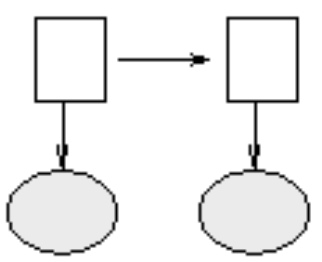
\includegraphics[scale=0.5]{E_1}
    \centering
\end{figure}
Define plausible expressions for the probabilities of initial, transition
and emission states, specifying their parameters. So suppose you have a
sequence \(Y=\{Y_1,...,Y_T\}\). Determine an expression for the likelihood
function:
\begin{align*}
    L(\theta)=p(S_{1:T}, Y_{1:T}|\theta)
\end{align*}

\Answer[number={1}]
Let's recall the HMM formula:
\begin{align*}
    Pr(S_{1:T}, y_{1:T}|\theta)
    &=Pr(S_1)\prod_{t=1}^{T}Pr(y_t|S_t)\prod_{t=2}^{T}Pr(S_t|S_{t-1})\\
    &=\text{initial state probability}\cdot\text{emission probability}\cdot\text{state transition probability}
\end{align*}
Notice that two states are available: \(s_1\) and \(s_2\). Moreover, the
probability that initial state \(S_1=s_1\) is \(\pi_1=p\), while the probability
that \(S_1=s_2\) is \(\pi_2=1-p\), leading to
\(\pi=[\pi_1\quad\pi_2]=[p\quad{1-p}]\).\\
Then, the initial state probability can be written as:
\begin{align*}
    P(S_1=s_i)
    =\prod_{i=1}^{2}\pi_i^{S_{1,i}}
    =\pi_1^{S_{1,1}}\cdot\pi_2^{S_{1,2}}
    =p^{S_{1,1}}\cdot(1-p)^{S_{1,2}}
\end{align*}
\begin{align*}
    \Rightarrow
    \log{Pr(S_1=s_i)}
    =\sum_{i=1}^{2}\log{\pi_i}^{S_{1,i}}
    =S_1^T\log{\pi}
\end{align*}
At this point, let's express the state transition probability as:
\begin{align*}
    Pr(S_t=s_t|S_{t-1}=s_{t-1})
    =\prod_{i=1}^2\prod_{j=1}^2(\phi_{ij})^{S_{t,i}\cdot S_{t-1,j}}
\end{align*}
\begin{align*}
    \Rightarrow
    \log{Pr(S_t=s_t|S_{t-1}=s_{t-1})}
    =\sum_{i=1}^2\sum_{j=1}^2S_{t,i}\cdot S_{t-1,j}\log{\phi_{ij}}
    =S_t^T\log{(\Phi)}S_{t-1}
\end{align*}
Finally, the emission probability can be written as follow, since the
observable nodes are Gaussian:
\begin{align*}
    p(y_t=y|S_t=s_i)
    =(2\pi)^{-\frac{d}{2}}|\Sigma|^{-\frac{1}{2}}\exp{\biggl\{-\frac{1}{2}(y_t-\mu)^T\Sigma^{-1}(y_t-\mu)\biggr\}}
\end{align*}
\begin{align*}
    \Rightarrow
    \log{p(y_t=y|S_t=s_i)}
    =-\frac{d}{2}\log{(2\pi)}-\frac{1}{2}\log{|\Sigma|}-\frac{1}{2}(y_t-\mu)^T\Sigma^{-1}(y_t-\mu)
\end{align*}
Henceforth:
\begin{align*}
    \log{Pr(S_{1:T}, y_{1:T}|\theta)}
    &=\log{Pr(S_1)}+\sum_{t=1}^{T}\log{Pr(y_t|S_t)}+\sum_{t=2}^{T}\log{Pr(S_t|S_{t-1})}\\
    &=S_1^T\log{\pi}+\sum_{t=1}^{T}\biggl[-\frac{d}{2}\log{(2\pi)}-\frac{1}{2}\log{|\Sigma|}-\frac{1}{2}(y_t-\mu)^T\Sigma^{-1}(y_t-\mu)\biggr]+\\
    &\quad +\sum_{t=2}^{T}S_t^T\log{(\Phi)}S_{t-1}
\end{align*}